\documentclass[12pt]{article}
\usepackage{amsmath}
\usepackage{array}
% \usepackage{gensymb}
\usepackage{geometry}
\usepackage{graphicx}
\usepackage{pgfplots}
\usepackage{siunitx}
\usepackage{wrapfig}

\title{Homework \#8}
\author{Donald Aingworth IV}
\date{October 16, 2024}

\pgfplotsset{width=8cm,compat=1.9}
\usepgfplotslibrary{external}
% \tikzexternalize

\begin{document}

\DeclareSIUnit{\mile}{mi}
\DeclareSIUnit{\gal}{gal}
\DeclareSIUnit{\foot}{ft}
\DeclareSIUnit{\h}{h}

\maketitle
\pagebreak
\section*{Problem 1}
A 0.315-kg particle moves from an initial position $\vec{r}_1$ = $2.00 \hat{i} - 1.00 \hat{j} + 3.00 \hat{k}$ m to a final position $\vec{r}_2 = 4.00 \hat{i} - 3.00 \hat{j} - 1.00 \hat{k}$ m while a force $\vec{F} = 2.00 \hat{i} - 3.00 \hat{j} + 1.00 \hat{k}$ N acts on it. What is the work done by the force on the particle?

\subsection*{Solution}


% \pagebreak
% \section*{Problem 2}
% Compute the kinetic energy for each of the cases below. Through what distance would a 800-N force have to act to stop each object? (a) A 150-g baseball moving at 40 m/s; (b) a 13-g bullet from a rifle moving at 635 m/s; (c) a 1500-kg Corvette moving at 250 km/h; (d) a $1.8 \times 10^5$ kg Concorde airliner moving at 2240 km/h.


% \subsection*{Solution}


% \pagebreak
% \section*{Problem 3}
% Compute the kinetic energies for each of the following. What force would be required to stop each object in 1.00 km? (a) The $8.00 \times 10^7 \unit{\kilo\gram}$ carrier Nimitz moving at 55 km/h; (b) a $3.4 \times 10^5 \unit{\kilo\gram}$ Boeing 747 moving at 1000 km/h; (c) the 270-kg Pioneer 10 spacecraft moving at 51,800 km/h.

% \subsection*{Solution}


% \pagebreak
% \section*{Problem 4}

% \begin{wrapfigure}{r}{0.25\textwidth}
%     \vspace{-25pt}
%     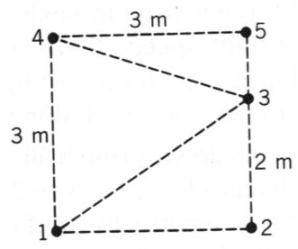
\includegraphics[width=0.25\textwidth]{graph_4.png} 
% \end{wrapfigure}
% A 1.50-kg block is moved at constant speed in a vertical plane from position 1 to position 3 via several routes shown in the figure. Compute the work done by gravity on the block for each segment indicated, where $W_{ab}$ means work done from a to b. (a) $W_{13}$, (b) $W_{12}$ + $W_{23}$ (c) $W_{14}$ + $W_{43}$, (d) $W_{14}$ + $W_{45}$ + $W_{53}$.

% \subsection*{Solution}


% \pagebreak
% \section*{Problem 5}
% What is the work needed to lift 14.7 kg of water from a well 11.0 m deep. Assume the water has a constant upward acceleration of 0.700 m/s$^2$.

% \subsection*{Solution}


% \pagebreak
% \section*{Problem 6}

% \begin{wrapfigure}{r}{0.25\textwidth}
%     \vspace{-50pt}
%     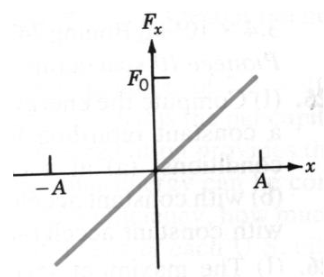
\includegraphics[width=0.25\textwidth]{graph_6.png} 
%     % \label{fig:wrapfig}
% \end{wrapfigure}
% The variation of a force with position is shown in the figure below. Find the work from (a) x = 0 to x = -A (b) x = +A to x = 0

% \subsection*{Solution}


% \pagebreak
% \section*{Problem 7}

% Consider a particle on which several forces act, one of which is known to be constant in time: $\vec{F}_1$ = 3.00 $\hat{i}$ + 4.00 $\hat{j}$ N. As a result, the particle moves along a straight path from a Cartesian coordinate of (0.00 m, 0.00 m) to (5.00 m, 6.00 m). What is the work done by $\vec{F}_1$?

% \subsection*{Solution}


% \pagebreak
% \section*{Problem 8}
% A bungee cord exerts a nonlinear elastic force of magnitude $F(x) = k_1x + k_2 x^3$, where $x$ is the distance the cord is stretched, $k_1 = 204 \unit{\N/\m}$ and $k_2 = -0.233 \unit{\N/\m^3}$. How much work must be done on the cord to stretch
% it 16.7 m?

% \subsection*{Solution}



\end{document}